\documentclass[runningheads]{llncs}
\usepackage{graphicx} % Required for inserting images
\usepackage{color}
\usepackage{amsmath}
\usepackage{pgfplots}
\usepackage{tikz}
\pgfplotsset{compat=1.18} 
\usetikzlibrary{matrix}
\usepackage{booktabs}

\makeatletter
\newenvironment{customlegend}[1][]{%
    \begingroup
    % inits/clears the lists (which might be populated from %previous
    % axes):
    \pgfplots@init@cleared@structures
    \pgfplotsset{#1}%
}{%
    % draws the legend:
    \pgfplots@createlegend
    \endgroup
}%

\def\addlegendimage{\pgfplots@addlegendimage}
\makeatother


\newcommand{\rev}{{\hat{~}}}
\newcommand{\U}{\mathcal{U}}
\newcommand{\V}{\mathcal{V}}
\newcommand{\dd}{\mathinner{.\,.}}
\newcommand{\rank}{\mathsf{rank}}
\newcommand{\select}{\mathsf{select}}

\newcommand{\dom}[1]{\ensuremath{\mathsf{dom}(#1)}}
\newcommand{\vars}[1]{\ensuremath{\mathsf{vars}(#1)}}
\newcommand{\lab}[1]{\ensuremath{\mathsf{word}(#1)}}

\newcommand{\inv}[1]{\ensuremath{\textsc{\^{}}#1}}
\newcommand{\comp}[1]{\ensuremath{#1^{\leftrightarrow}}}
\newcommand{\dinv}[1]{\ensuremath{#1^{--}}}

\newcommand{\diego}[1]{{\color{red}\textsc{Diego:} #1}}
\newcommand{\gonzalo}[1]{{\color{green!50!black}\textsc{Gonzalo:} #1}}
\newcommand{\adrian}[1]{{\color{brown!90!black}\textsc{Adrian:} #1}}

\newcommand{\update}[1]{{\color{red}#1}}




\title{Evaluating Regular Path Queries \\ on Compressed Adjacency Matrices\thanks{\tiny This work was supported by ANID – Millennium Science Initiative Program – Code ICN17\_002, and Fondecyt Grant 1-230755, Fondecyt Grant 1221926; 
CITIC is funded by Xunta de Galicia and CIGUS; GAIN/Xunta de Galicia Grant ED431C 2021/53 (GRC); Xunta de Galicia/FEDER-UE Grant IN852D 2021/3; MCIN/AEI and NextGenerationEU/PRTR Grants [PID2020-114635RB-I00, TED2021-129245B-C21]
}}
\author{Diego Arroyuelo\inst{1,2} \and Adrián Gómez-Brandón\inst{1,3} \and Gonzalo Navarro\inst{1,4}}

\institute{
Millennium Institute for Foundational Research on Data (IMFD)
\and 
Department of Informatics, Universidad T\'ecnica Federico Santa Mar\'ia, Chile
\and 
CITIC Research Center, Universidade da Coruña, Spain
\and
Department of Computer Science, University of Chile, Chile}

\begin{document}

\maketitle

\begin{abstract}
Regular Path Queries (RPQs), which are essentially regular expressions to be matched against the labels of paths in labeled graphs, are at the core of graph database query languages like SPARQL. A way to solve RPQs is to translate them into a sequence of operations on the adjacency matrices of each label. We design and implement a Boolean algebra on sparse matrix representations and, as an application, use them to handle RPQs. Our baseline representation uses the same space as the previously most compact index for RPQs and excels in handling the hardest types of queries. Our more succinct structure, based on $k^2$-trees, is 4 times smaller and still solves complex RPQs in reasonable time.
\end{abstract}

\section{Introduction and Related Work}

Graph databases have emerged as a crucial tool in several applications such as web and social networks analysis, the semantic web, and modeling knowledge, among others. We are interested in labeled graph databases, where the graph edges have labels. One particular way of querying graph databases is by means of basic graph patterns (BGPs, for short), which are small subgraphs with constant or variable nodes and edge labels that are to be matched homomorphically in the graph database. 
%In our example, the BGP $\{ \mathtt{?x} \xrightarrow{\mathsf{walk}} \mathtt{?y},~ \mathtt{?y} \xrightarrow{\mathsf{walk}} \mathtt{?z},~ \mathtt{?z} \xrightarrow{\mathsf{walk}} \mathtt{?x} \}$ looks for three places within walking distance to each other.
BGPs are strongly related to relational database joins \cite{HoganRRS19}. Another important kind of queries that are more exclusive of graph databases are the \emph{regular path queries} (RPQs, for short), which search for paths of arbitrary length matching a regular expression on their edge labels \cite{AnglesABHRV17}. For example, in the simple RDF model \cite{rdf}, one can represent points of interest in New York City as nodes in a graph, and have edges such as $x \xrightarrow{\mathsf{walk}} y$ indicating that $x$ is within a short walking distance of $y$, as well as edges of the form $x \xrightarrow{\mathsf{L}} y$ if subway stations $x$ and $y$ are connected directly by subway line $\mathsf{L}$. Then the RPQ
`$\text{Central Park}~\mathsf{walk}/(\mathsf{N} | \mathsf{Q} | \mathsf{R})^+/\mathsf{walk}~\mathtt{?y}$',
asks for all sites $\mathtt{?y}$ of interest that are reachable from Central Park by using subway lines \textsf{N}, \textsf{Q}, or \textsf{R}, through one or more stations and allowing a short walk before and after using the subway.


%Mention that RPQs appear in various query languages such as SPARQL, GQL (?), ...  \cite{GQL}
RPQs are at the core of current graph database query languages, extending their expressiveness. In particular, the SPARQL 1.1 standard includes the support for \emph{property paths}, that is, RPQs extended with inverse paths (known as two-way RPQs, or 2RPQs for short) and negated label sets. As SPARQL has been adopted by several systems, RPQs have become a popular feature~\cite{AnglesABHRV17}: out of 208 million SPARQL queries in the public logs from the Wikidata Query Service~\cite{MalyshevKGGB18}, about 24\% use at least one RPQ feature~\cite{BonifatiMT19}. Further developments like PGQL~\cite{RestHKMC16}, Cypher~\cite{FrancisGGLLMPRS18}, G-CORE~\cite{AnglesABBFGLPPS18}, TigerGraph~\cite{DeutschXWL20}, and GQL~\cite{GQL}, to name some of the most popular ones, also support RPQ-like features. 
%So, efficiently managing RPQs is crucial for the systems supporting these languages. 


%Several approaches to handle RPQs, esp. the product graph.
Handling (2)RPQs can be computationally expensive to evaluate as they usually involve a large number of paths \cite{MartensNPRVV23}, mostly for regular expressions using Kleene stars. There are two main algorithmic approaches to support them \cite{YakovetsGG16}: (1) to represent the regular expression of the 2RPQ using a finite automaton, which is then used to search over the so-called product graph~\cite{MendelzonW95}; and (2) to extend the relational algebra to support computing the transitive closure of binary relations to evaluate regular expressions having Kleene stars \cite{LMpods12}. Although most theoretical results on 2RPQs have followed the first approach, property path evaluation in SPARQL has followed the second one \cite{YakovetsGG16}.   


%Recent approaches to compressed data structures, our ICDE paper.

Recent research introduced not only time- but also space-efficient solutions for evaluating graph joins~\cite{ANRRtods22,AHNRRS21,BCdBFNsupe22}. With the big graphs available today, this is an important step towards in-memory processing of graph queries. In particular, the Ring data structure~\cite{AHNRRS21} is able to represent a labeled graph in space close to its plain representation, while supporting worst-case optimal joins (used, as we said, for BGP queries).  Moreover, by using little extra space the Ring can be used to support 2RPQs efficiently \cite{AHNRicde22}, using the product-graph approach~\cite{MendelzonW95}. 



%Alternative approach based on matrix operations: Boolean sum, Boolean multiplication, transitive closure.  Find a reference on this, I guess it exists... \diego{Losemann y Martens basan la evaluación en algebra de matrices, excepto para la concatenación que la hacen con un join. Sin embargo, es un paper teorico sobre la complejidad de evaluar RPQs, no dice mucho de la implementacion.}
%Typically disregarded because matrices are huge, but otoh they tend to be sparse.
%We explore this approach: translate RPQs into operations on sparse matrices. Those are represented with the well-known k2tree. We show how to do this translation and handle the particularities of RPQs. The result is the most succinct graph db representation ( 5.x bpt in our wikidata experiments) while being competitive with approaches that use much more space. 

In this paper, we introduce a space-efficient approach for evaluating 2RPQs that, essentially, represents the subgraph corresponding to each graph label $p$ using a sparse representation of its Boolean adjacency matrix $M_p$. We evaluate 2RPQs by translating them into classic operations on Boolean matrices \cite{LMpods12}.
%(such as, e.g., sums, products, and transitive closures). 
This approach is typically disregarded because matrix sizes are quadratic on the number of graph nodes, but we exploit the sparsity of those matrices to represent them efficiently, using $k^2$-trees \cite{BLNis13}. The use of $k^2$-trees to represent each RDF predicate is not new, for example it has been used to handle triple matching and binary joins \cite{AGBFMPN13} and full BGPs \cite{ANRRtods22}, but not 2RPQs. We show how to translate 2RPQs into matrix operations and how to handle the particularities of 2RPQs. 

The result is the most space-efficient graph database representation (nearly 4 bytes per graph edge on a Wikidata graph, 4 times less than the previously most compact representation---the Ring \cite{AHNRicde22}---and 14--21 times smaller than classical systems). In exchange, our structure is on average 5 times slower than the Ring, though it still solves most complex 2RPQs in a few seconds. 
%Our new structure and the Ring now dominate the space-time tradeoff map. 
We also implement an uncompressed baseline for sparse matrices based on the CSR and CSC formats \cite[Sec.~3.4]{Saa03}. Its space matches that of the Ring and it excels on the most expensive 2RPQs, namely those where no graph node is specified. It is only outperformed by Blazegraph, which uses 5.5 times more space. Our new matrix-algebra-based approach stands out in the space-time tradeoff map.

\section{Basic Concepts}


\subsection{Labeled Graphs and Regular Path Queries (RPQs)} 

See Appendix~\ref{sec:labeled-graphs-rpqs} for the formal definitions.

\subsection{An Algebra on Boolean Matrices} \label{sec:matrix-algebra}

%Define the Boolean operations $A+B$, $A\times B$, $A^*$, $A^+$, and some extensions we will need: $A^T$, $[row]A$, and $A[col]$. The last two return a matrix of the same dimensions of $A$ but with only that row or col, the rest are zeros.

Let $A=(a_{i,j})_{1\le i, j\le n}$ and $B = (b_{i,j})_{1\le i, j\le n}$ be square $n\times n$ Boolean matrices. We define the following operations of interest for our work: %\gonzalo{Mencionar la notación $a_{i,j}$ para $A$}
\begin{itemize}
    \item \textbf{Transpose}: $A^T$, where $a^T_{i,j} = a_{j,i}$, for $1\le i, j\le n$.
    \item \textbf{Sum}: $A+B = C=(c_{i,j})$, where $c_{i,j} = a_{i,j} \vee b_{i,j}$, for $1\le i, j\le n$.
    \item \textbf{Product}: $A\times B = C$, where for $1\le i, j\le n$ we have $c_{i,j} = \bigvee_{1\le k\le n}{a_{i,k} \wedge b_{k,j}}.$
    \item \textbf{Exponentiation}: $A^k = \prod_{i=1}^{k}{A}$, that is, $A \times \cdots \times A$, writing $A$ $k$ times. % (A^{k/2})^2$, which takes $\lg{k}$ multiplications.
    \item \textbf{Transitive closure}: $A^+ = A+A^2+\cdots + A^n$.
    \item \textbf{Reflexive-transitive closure}: $A^* = I + A^+$, where $I$ is the identity matrix.
    \item \textbf{Row restriction}: $\langle r\rangle A$, a matrix whose row $r$ equals row $r$ of $A$, the remaining cells are $0$.
    \item \textbf{Column restriction}: $A\langle c\rangle$, a matrix whose column $c$ equals column $c$ of $A$, the remaining cells are $0$. 
    \item \textbf{Cell restriction}: $\langle r\rangle A\langle c\rangle$, a matrix whose cell $(r,c)$ equals entry $A[r][c]$, the remaining cells are $0$.
\end{itemize}

The implementation of these operations on sparse matrix representations is relatively straightforward, except for the multiplication and transitive closures. See Appendix~\ref{sec:clausura} for a brief survey on known algorithms for those.



\subsection{$K^2$-trees} \label{sec:k2trees}

%As a tool to represent sparse Boolean matrices. For $k=2$. Implemented over LOUDS-like. Explain the z-order, 0123 for top-left, top-right, bottom-left, bottom-right. Give the name signature to the 4 bits that describe each node.

A $k^2$-tree \cite{BLNis13} is a data structure able to space-efficiently represent binary relations, point grids, and graphs. We will use it in this paper to represent Boolean matrices, as follows. Let $A$ be a $v \times v$ Boolean matrix, assuming $v$ is a power of 2.\footnote{If $v$ is not a power of 2 we round it up to the next power, leaving the extended cells empty. This imposes almost no extra overhead on the $k^2$-tree representation.} The root node of the $k^2$-tree represents the whole matrix $A$. Then, $A$ is divided into 4 equally-sized quadrants, $A = {A_0 ~ A_1 \choose A_2 ~ A_3}$, such that submatrix $A_0$ is represented recursively by the first child of the root, $A_1$ by the second child, and so on. The process stops as soon as one gets into an empty submatrix, which is represented by a leaf node. Each node in this tree has 4 children (in general, $k^2$ children, yet we use $k=2$). This order in which quadrants are represented (i.e., top-left, top-right, bottom-left, and bottom-right) is known as z-order. The resulting tree height is $\log_4 v^2 = \log_2 v$. 

To represent this tree space-efficiently, we traverse the tree in level order. At each node, we write its 4-bit signature (which represents the node) indicating whether each of the 4 children represents an empty submatrix or not. For instance, the signature \texttt{0110} indicates that quadrants $0$ and $3$ of the submatrix represented by the current node are empty, whereas $A_1$ and $A_2$ (second and third children) are non-empty. The result is a bit vector $L[1\dd 4n]$, where $n$ is the number of internal nodes in the tree. Each tree node is represented by the first bit of its signature. Given a node $i$, its $j$-th child ($0\le j\le 3$) is represented at position $4\cdot\rank_1(L, i) + 1$, where $\rank(L, i)$ counts the number of 1s in $L[1\dd i]$ in $O(1)$ time using $o(n)$ additional bits of space \cite{Cla96,Mun96}. 

The $k^2$-tree representation is especially useful for representing sparse matrices. Let matrix $A$ have $a$ 1s. Then, in the worst case every 1 induces a 4-bit signature in every level of the $k^2$-tree, for a total of $4a\log_2 v$ bits. The actual upper bound is lower because not all those signatures can be different: in the worst case all the
$k^2$-tree nodes up to level $\lfloor \log_4 a \rfloor$ exist, and from there on each 1 of $A$ has its own path; this adds up to $4a\log_4(v^2/a)+4a/3+O(1)$ bits. The figures further improve when the 1s are clustered in $A$ \cite{dBGLNSjcss22}.

%We note that constant-time $\rank$ is possible in the so-called transdichotomous RAM model of computation, where we assume that the computer word holds $\Omega(\log v)$ words in order to represent $\log_2 v$-bit coordinates in $O(1)$ words (and thus handle them in $O(1)$ time). We assume this computation model as well.

\section{Evaluating RPQs through the Boolean Matrix Algebra} \label{sec:evaluating-rpqs}

For a given directed edge-labeled graph $G$ of $n$ edges, let $P$ be the corresponding set of graph labels as defined in Section \ref{sec:labeled-graphs-rpqs}. In our approach, for every $p \in P$ we define a $|V|\times |V|$ Boolean matrix $M_p$, such that $M_p[x][y] = 1$ iff $(x, p, y) \in G$. We translate an RPQ into operations on those matrices, so that the resulting Boolean matrix contains all pairs $(x, y)$ that match the regular expression. 
We define next the recursive formulas ${\cal M}$ to translate 2RPQs into matrix operations, following Losemann and Martens' work \cite{LMpods12}. We start with the base cases: 
\begin{itemize}
    \item ${\cal M}(\varepsilon) = I$, the identity matrix.
    \item ${\cal M}(p) = M_{p}$, for $p \in P$. 
    \item ${\cal M}(\rev p) = M_{p}^T$, for $p \in P$.
\end{itemize}
Next, let $E_1$ and $E_2$ be 2RPQs. We define the following recursive rules: 
\begin{itemize}
    \item ${\cal M}(E_1 ~|~ E_2) = {\cal M}(E_1) + {\cal M}(E_2)$
    \item ${\cal M}(E_1 / E_2) = {\cal M}(E_1) \times {\cal M}(E_2)$
    \item ${\cal M}(E_1^+) = {\cal M}(E_1)^+$
    \item ${\cal M}(E_1^*) = I + {\cal M}(E_1)^+$, where $I$ is the corresponding identity matrix.
\end{itemize}
Then, given a 2RPQ $R = (x,E,y)$, we evaluate it as follows:
\begin{enumerate}
    \item If $x$ and $y$ are both variables, ${\cal R}(R) = {\cal M}(E)$
    \item If $x$ is a variable and $y$ is a constant, ${\cal R}(R) = {\cal M}(E)\langle y\rangle$
    \item If $x$ is a constant and $y$ is a variable, ${\cal R}(R) = \langle x\rangle{\cal M}(E)$
    \item If $x$ and $y$ are both constant, ${\cal R}(R) = \langle x\rangle{\cal M}(E)\langle y\rangle$
\end{enumerate}

\section{Implementation of the Boolean Matrix Algebra}

We now describe how the Boolean-matrix operations are carried out. To analyze the corresponding algorithms, we use $|M_{p}|$ as the number of 1s in the matrix, which is the number of edges with label $p$ in graph $G$. 
We represent each matrix $M_p$ using a $k^2$-tree of $O(\log |V|)$ levels, and each 1 in $M_p$ induces $O(\log |V|)$ 1s in its $k^2$-tree representation. We will use $v=|V|$, as well as $a=|A|$ and $b=|B|$ for the number of 1s in matrices $A$ and $B$. We assume $|V| = 2^i$, for $i \ge 0$.

We implement $k^2$-trees, and thus bitvectors with $\rank$ support, from scratch. We store the bitvector as consecutive bits packed in a 64-bit-words array. To support $\rank$ we store the cumulative sum of 1s up to every $s$th cell of the array. To save space, full 64-bit integers store the full sum only every $2^{16}$ bits, and the others are stored in relative form using 16-bit integers. To compute $\rank$ we start from the last recorded sum and use {\em popcount} on the full words until reaching the desired one, and a partial {\em popcount} on the desired word. Here $s$ is a space-time tradeoff parameter: we use $n/1024+n/(4s)$ additional bits of space for storing a bitvector $B[1\dd n]$, and compute $\rank$ in time $O(s)$. We use $s=4$.

\subsection{Transposition}

Transposition is used to implement reversed edges, as seen in Section \ref{sec:evaluating-rpqs}. Instead of materializing the transposed matrix as a $k^2$-tree, we note that $A^T = {A_0^T~A_2^T \choose A_1^T~A_3^T}$.
%$$ A^T =
%\Biggl(\mkern-5mu
%\begin{tikzpicture}[baseline=-.65ex]
%\matrix[
%  matrix of math nodes,
%  column sep=1ex,
%] (m)
%{
%A_0^T & A_2^T \\
%A_1^T & A_3^T\\
%};
%\draw[dotted]
%  ([xshift=0.5ex]m-1-1.north east) -- ([xshift=0.5ex]m-2-1.south east);
%\draw[dotted]
%  (m-1-1.south west) -- (m-1-2.south east);
%\end{tikzpicture}\mkern-5mu
%\Biggr).$$
So, the $k^2$-tree for $A^T$ can be obtained by interchanging the roles of the second and third children of every node. We do not materialize this interchange,  but associate a {\em transposed} flag to every matrix, so we simply have to toggle it in order to transpose the matrix in $O(1)$ time.




\subsection{Boolean Sum} \label{sec:sum}

The easier case to implement $A+B$ arises when no matrix is transposed. In this case we can perform a sequential pass over both $k^2$-tree bitvectors, so as to merge their corresponding nodes levelwise, without need of any $\rank$ operation. 

We implement this traversal with a queue of tasks, which are of two types. (\emph{1}) A {\em copy} task indicates just to copy the next node from $A$ or $B$; and (\emph{2}) a {\em merge} task indicates merging the next nodes of $A$ and $B$. The queue is initialized with a merge task, the read-pointers (which indicate the next $k^2$-tree node to be read) at the beginning of the bitvectors of $A$ and $B$, and the write-pointer at the beginning of the output $k^2$-tree bitvector.

To process a copy task, we append the next signature (of $A$ or $B$) to the output, and enqueue its (up to) 4 children, as copy tasks for $A$ or $B$, respectively. To process a merge task, we append to the output the bitwise-or of the next 4-bit signatures of $A$ and $B$, and enqueue up to 4 new elements, as follows. For $i$ from 1 to 4, if the $i$th bit of the signatures of both $A$ and $B$ are 1, we append a merge task. If only one of them is 1, we append a copy task for the corresponding matrix. If none is 1, we do not append a task.
We do not append new tasks when the corresponding nodes are $k^2$-tree leaves. The process finishes when the queue becomes empty. The total time is proportional to the sum of the bitvector length of both matrices, $O(a\log (v^2/a)+b\log(v^2/b)) \subseteq O((a+b)\log v)$.

\paragraph{Handling transpositions.} If both $A$ and $B$ are transposed, we just merge them as described and mark the result as transposed. When one is transposed and the other is not, we cannot anymore resort to a sequential traversal of both bitvectors. The transposed one must already have $\rank$ support built to enable $k^2$-tree traversals. We traverse sequentially the non-transposed $k^2$-tree, and include in the queue the corresponding node of the transposed one (as those nodes are not read in left-to-right order). To generate the new tasks, we must use the $k^2$-tree traversal operations to locate the corresponding nodes in the transposed $k^2$-tree. 

While the time complexity is the same, summing a transposed with a non-transposed matrix is slower in practice. We always choose that the transposed matrix is the one with a shorter bitvector (we can because $A^T+B = (A+B^T)^T$), in order to minimize the non-local traversals.

\subsection{Boolean Multiplication}

For the multiplication $A \times B$ we use the following classic divide-and-conquer recursive procedure. Let $A = { A_0~A_1 \choose A_2~A_3}$ and $B = { B_0~B_1 \choose B_2~B_3}$ be the four submatrices into which the $k^2$-tree representation splits $A$ and $B$. Then, we recursively compute 8 products of those submatrices in order to produce
%$$ A \times B ~~=~~ { A_0 \times B_0 + A_1 \times B_2 ~~~ A_0 \times B_1 + A_1 \times B_3
%                      \choose
%                     A_2 \times B_0 + A_3 \times B_2 ~~~ A_2 \times B_1 + A_3 \times B_3 }.
%$$
\begin{equation} \label{eq:matrix-multiplication}
A \times B = 
\Biggl(\mkern-5mu
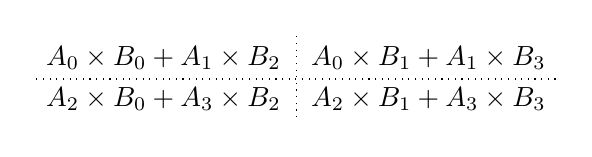
\begin{tikzpicture}[baseline=-.65ex]
\matrix[
  matrix of math nodes,
  column sep=1ex,
] (m)
{
A_0\times B_0 + A_1\times B_2 & A_0\times B_1 + A_1\times B_3 \\
A_2\times B_0 + A_3\times B_2 & A_2\times B_1 + A_3\times B_3 \\
};
\draw[dotted]
  ([xshift=0.5ex]m-1-1.north east) -- ([xshift=0.5ex]m-2-1.south east);
\draw[dotted]
  (m-1-1.south west) -- (m-1-2.south east);
\end{tikzpicture}\mkern-5mu
\Biggr).
\end{equation}
A fortunate consequence of the $k^2$-tree representation is that, if any of those submatrices is empty (i.e., there is a 0 in the signature of the root of $A$ or $B$), then we know that its product with any other submatrix is also zero. Further, summing a product $A_i \times B_j$ with a zero matrix does not even need to copy the product; we just reference it as the final result.

Once the $k^2$-tree bitvectors of the four submatrices are recursively obtained, we concatenate them levelwise. There is no need to build the $\rank$ data structures until we obtain the final matrix because the concatenation proceeds left-to-right in each level. We only take care of maintaining, for each bitvector, $O(\log v)$ pointers to the positions where the levels start.

Transpositions are handled easily, by exchanging the meaning of $M_1$ and $M_2$ in every node of the $k^2$-tree bitvector if $M = { M_0~M_1 \choose M_2~M_3}$is transposed.

\paragraph{A rough analysis.}
One term of the multiplication cost is given by the number of recursive calls, which follows the recurrence
$T(v^2) = 8 \cdot T(v^2/4)$. Since our matrices are sparse, the worst case arises when every submatrix has points up to the level $\ell$ where we have $4^\ell \ge \min(a,b)$ submatrices, that is, $\ell = \log_4 \min(a,b)$. From this level, the worst case is that the $\max(a,b)/\min(a,b)$ points in the submatrices of the fuller matrix distribute uniformly for $\ell' = \log_4 \frac{\max(a,b)}{\min(a,b)}$ further levels. Between those levels, the recurrence becomes $T'(v^2) = 2 \cdot T'(v^2/4)$ because the single point in the emptier submatrix can make us enter into at most two submatrices of the other. This continues until, in level $\ell+\ell'$, both submatrices contain one point each, and from there on the cost is just $\log_2 v - \ell-\ell'$ to track a single point along both submatrices. The cost up to level $\ell$ is then $8^{\ell} = \min(a,b)^{3/2}$. From each of those $8^{\ell}$ submatrices we have a cost of $2^{\ell'} = (\max(a,b)/\min(a,b))^{1/2}$, and from each of those $8^{\ell} 2^{\ell'} = \min(a,b)\sqrt{\max(a,b)}$ submatrices we have $O(\log (v^2/\max(a,b)))$ additional time. The total cost of recursive calls is then $O(\min(a,b)\sqrt{\max(a,b)}\log (v^2/\max(a,b)))$. 

The second part of the cost is that of summing pairs of partial submatrices. In the worst case, those matrices may add up to $a \cdot b$ points at across every level $\ell$ of the recursion. Since summing submatrices in level $\ell$ costs $O(\ell)$ per element, the total cost of summing partial results is in $O(ab\log^2 v)$. Since this is an utterly pessimistic upper bound, we offer an average-case time analysis for matrices with uniformly distributed 1s. We multiply $8^\ell$ pairs of $v/2^\ell \times v/2^\ell$ submatrices in level $\ell$. On average, each has $a/4^\ell$ 1s in $A$ and $b/4^\ell$ cells in $B$. Every such $a_{ik}$ will pair with every such $b_{k'j}$ iff $k=k'$, which occurs with probability $1/(v/2^\ell)$, so on average there will be $8^\ell (a/4^\ell)(b/4^\ell)(2^\ell/v) = ab/v$ 1s to sum per level $\ell$, with a maximum of $v^2$. This leads to a total average cost upper bounded by
$O(\min(a,b)\sqrt{\max(a,b)}\log v + \min(v^2,(ab/v))\log^2 v)$.

\subsection{Closure}

We opted for a simple transitive closure algorithm for now.
The closure $A^+$ is obtained by iteratively computing 
$A \gets A + A \times A$ until no change occurs in $A$ \cite{Furman70}. This occurs at most after $\log_2 v$ iterations, so the time complexity is $O(\log v)$ times that of multiplying $A$ by itself (note that $a$ grows in every iteration, so the time complexity becomes bounded by $O(|A^+|^{3/2}\log^3 v)$). 
The transitive closure is computed as $A^* = I + A^+$, where $I$ is the identity matrix. 

Needless to say, unrestricted closure operations are the most expensive, both in time complexity and in practice, so we aim to avoid them as much as possible.

\subsection{Restrictions}\label{sec:restrictions}

Restrictions indicate that we only want to retrieve a column or a row of the matrix after the operations, or even just a cell. A naive way to implement them is to first obtain the full matrix $M$ and then traverse the desired row or column. Yet, restrictions give an important opportunity of optimizing all the other operations. 

\paragraph{Sums.} For $\langle r\rangle (A+B)\langle c\rangle $ (where only $\langle r\rangle $ or only $\langle c\rangle $ could be present as well), we restrict the traversal of both matrices, acting as if the submatrices not intersecting the desired row and/or columm were empty. That is, we implement the restricted sum as $\langle r\rangle A\langle c\rangle  + \langle r\rangle B\langle c\rangle $. We cannot, however, simply traverse both $k^2$-tree bitvectors and write the output left-to-right, as in Section~\ref{sec:sum}, because now we do not know beforehand whether a submatrix (or the merge of two submatrices) will be nonempty after restricting it to some row/column, even if it intersects the row/column. Our solution is then recursive, similar to the multiplication algorithm (yet still considerably simpler). 
%Letting $c$ be the number of points in the restricted matrix, if only a row or a column is restricted (so $c \le \min(v,a+b)$), we recurse on two submatrices, thus the recurrence for the time complexity is $T(v^2) = 2 \cdot T(v^2/4) + c + \log v$. Considering as before the worst case where we recurse for $\log_2 c$ levels until every submatrix has a single element, this solves to $T(v^2)=O((c+\log (v^2/c))\log v) \subseteq O((c+\log v)\log v$. This can be reduced to $O(c\log v)$ by merging the lower submatrices only every $\frac{1}{2}\log v$ levels. If both row and column are restricted, the time is just $O(\log v)$.

\paragraph{Products.}
A restricted product $\langle r\rangle  (A \times B) \langle c\rangle $ is handled as $(\langle r\rangle A) \times (B\langle c\rangle )$, where again only one of the restrictions may be present. We consider the column or row restrictions along the whole recursion, pretending that the submatrices that do not intersect the desired row or column are empty. %Having only one restriction modifies the recurrence of the product cost to $T(v^2) = 6 \cdot T(v^2/4) + c +\log v$, which solves to $T(v^2) = O((\min(a,b)^{\frac{1}{2}\log_2 6}+c+\log v)\log v)$, where $\frac{1}{2}\log_2 6 < 1.3$ and we note that $\min(a,b),c \le v$. Having both restrictions yields $T(v^2) = 4 \cdot T(v^2/4) + c +\log v$, which solves to $T(v^2) = O((\min(a,b)+c+\log v)\log v)$.

\paragraph{Closures.}
Operation $A^+\langle c\rangle $ is implemented as
$S \gets (E + A)\langle c\rangle $, where $E$ is the empty matrix, and then repeatedly doing $P \gets A \times S$ and $S \gets S + P$ until $S$ does not change. Note that the only nonzero column of $P$ and $S$ is $c$. To implement $A^*\langle c\rangle $ we start with $S = (I + A)\langle c\rangle$ instead. 
A row restriction $\langle r\rangle A^+$ is handled analogously, starting with $S = \langle r\rangle (A + E)$ and then iterating over $P \gets S \times A$ and $S \gets S + P$, or using the initial step $S \gets \langle r\rangle  (I + A)$ for $\langle r\rangle A^*$. 

Note that this iteration does not make the path lengths grow exponentially for the transitive closure, but linearly. Therefore, we could need up to $v$ iterations to compute the closure. In practice, the closure is reached much sooner and the operations are significantly faster, leading to a much better solution. 

When both row and column are restricted, we only want a cell of the transitive closure. We then choose the row/column with fewer elements in $A$ and run a row-restricted or column-restricted closure, whichever is emptier. At each step, we check if the desired cell is full, stopping immediately if so.

\subsection{Query Plan}

We first build the syntax tree of the 2RE $E$ of the 2RPQ $(x,E,y)$. In principle, we can simply traverse the syntax tree and solve it in postorder in the standard way, interpreting the leaves $p$ as the matrix $M_p$, $\rev p$ as $M_p^T$, and $\varepsilon$ as $I$, and interpreting the internal nodes as the corresponding operations on the matrices resulting from their children, according to the translations of Section~\ref{sec:evaluating-rpqs}. Our particular application, however, enables some relevant optimizations.

Let us first assume that both $x$ and $y$ are variables. A first simple optimization is that the closures are idempotent, so a sequence of closures is reduced to one. More precisely, $(A^*)^* = (A^*)^+ = (A^+)^* = A^*$ and $(A^+)^+ = A^+$. Sums and products yield more important optimizations, though. 
%Every regular expression $E$ can be represented using its syntax tree, a hierarchical binary tree structure that represents the relationships between its elements and operators. In the context of RPQs, each node $v$ stores an operator or a label, and its descending syntax (sub)tree describe the (sub)expression $E(v)$. Note that the root represents the whole expression $E$.
%
%\adrian{Figura con syntax tree}
%
%
% In order to solve $R=(x,E,y)$ our algorithm traverses the syntax tree of $E$ in postorder and translates each subexpression in Boolean-matrix operations according to the visited nodes and the translations of Section~\ref{sec:evaluating-rpqs}. 
%However, computing a subexpression $E(v)$ as soon as we solve its dependencies (i.e., every subexpression of the children of $v$ was solved) may not be a good option in certain cases because of its bad performance. For this reason, we propose a strategy that delays some operations until they are actually needed.
%
%Firstly, let us assume $R=(x, E, y)$ is not restricted, that is, $x$ and $y$ are variables. During the postorder traversal, the closures are solved once we reach an operator node because we cannot group them together. Note that having two consecutive closures in the regular expression, can be simplified to using the most restrictive one. With respect to the leaves, we just need to obtain the matrix of its label. Therefore, there are only two operations that can be delayed: sums and products. 

 \paragraph{Sums.} We exploit the fact that the Boolean sum is commutative and associative to carry out a sequence of consecutive sums, $E_1~| \dots|~ E_m$, in the best possible order. Since the cost of computing $A+B$ is proportional to $|A|+|B|$, if it were the case that $|A+B|=|A|+|B|$, the best possible order would be given by building the Huffman tree \cite{Huf52} of the matrices $A_i = {\cal M}(E_i)$ using $|A_i|$ as their weight. Since, instead, it holds that $\max(|A|,|B|) \le |A+B| \le |A|+|B|$, we opt for a heuristic that simulates Huffman's algorithm on the actual size of the matrices as they are produced. Concretely, we start with $\{ A_1, \ldots, A_m \}$ and iteratively remove from the set the two matrices $A_i$ and $A_j$ with the smallest sizes, sum them, and return $A_i + A_j$ to the set, until it has a single matrix.

%\paragraph{Sums.} The syntax tree can contain a node $v$ whose operator is $|$ and its $E(v)$ has the form $E_1~| \dots|~ E_m$, where $E_i$ is another regular expression. Note that ${\cal M}(E(v)) = {\cal M}(E_1) + \dots + {\cal M}(E_m)$. By following the postorder traversal we should solve ${\cal M}(E_{m-1})+{\cal M}(E_m)$ before the others, which can be expensive if the number of merge operations is large. Since the sum of matrices is commutative, we can delay that computation until we come back to $v$ and choose another order that minimizes the number of merge tasks. 
%
%The sum of two sparse matrices tends to be faster than in dense matrices because they need fewer merge tasks (e.g., the addition of an empty node with a non-empty one, requires a copy task). Therefore, we look for the two most sparse matrices $A$ and $B$ and compute $C=A+B$. Then, we replace both submatrices with $C$ and we repeat those steps until obtaining the final matrix, which is the result of $E(v)$. Detecting whose are the two most sparse matrices is easily computed by choosing those $A$ and $B$ that get the smallest $a$ and $b$, respectively.

\paragraph{Products.} Matrix multiplication is not commutative but still associative, so we can decide the order in which the sequence of multiplications to compute $E_1 ~/ \cdots /~ E_m$ is carried out. We cannot apply the well-known optimal algorithm to choose the order for dense matrices \cite[Sec.~15.2]{CLRS09} because the time complexity of our sparse matrix multiplications depends on the number of 1s in the matrices. Further, this number of 1s can increase or decrease after a multiplication. We then opt for a heuristic analogous to the one we use for sums: we start from the sequence $A_1,\ldots,A_m = {\cal M}(E_1),\ldots,{\cal M}(E_m)$ and iteratively choose the consecutive pair $A_i$, $A_{i+1}$ that minimizes $|A_i|+|A_{i+1}|$, multiply them, and replace the pair by $A_i \times A_{i+1}$, until the sequence has a single element.  

%\paragraph{Products.} Similar to the sums, we can find a node $v$ whose expression translation makes ${\cal M}(E(v)) = {\cal M}(E_1) \times \dots \times {\cal M}(E_m)$. Note that the product of two sparse matrices can generate a more sparse matrix. Therefore, delaying the products until we return to $v$ and multiplying first those that are the most sparse is a good option to solve $E(v)$ in an efficient way. 
%
%However, the product of matrices is not commutative, thus we need to respect the order of the matrices. For this reason, we look for the pair of consecutive matrices $A$ and $B$ that minimizes $\min(a, b)$. We compute the result $C=A \times B$, and replace both matrices with $C$. This procedure is recursively repeated until obtaining the final matrix.


\paragraph{Handling restrictions.}

When $x$ (resp., $y$) is a constant we are restricting a row (resp., column) of the matrix after the operations. For efficiency, then, we apply the restricted operations of Section~\ref{sec:restrictions}. Regarding the sums, because $\langle r\rangle (A+B) \langle c\rangle = \langle r\rangle A \langle c\rangle + \langle r\rangle B \langle c\rangle$, we can restrict all the involved matrices at the same time. Consequently, the sum can be computed in any order, and the plan still focuses on looking for the best order based on Huffman's algorithm. In the restriction on products, we obtain a sequence $\langle r\rangle A_1 \times \cdots \times A_m \langle c\rangle$ (where only $\langle r \rangle$ or only $\langle c \rangle$ could be present). Consider the case $\langle r\rangle A_1 \times \cdots \times A_m$. The number of 1s reduces faster when multiplying the pair that contains the restricted matrix, so we compute $A' = \langle r\rangle A_1 \times A_2$. The matrix $A'$ already has all zeros except in row $r$, so we can continue left-to-right in the sequence with normal matrix multiplications, $A' \times A_3$, and so on. The case $A_1 \times \cdots \times A_m \langle c\rangle$ is analogous, starting with $A' = A_{m-1} \times A_m \langle c\rangle$ and then completing the multiplications right to left. When both restrictions are present, we choose an end and proceed as explained until the final multiplication, $\langle r\rangle A' \times A'' \langle c\rangle$, which is carried out with the restricted multiplication algorithm to enforce the other restriction. 

Some restrictions can be inherited by the operands of a node, which speeds up processing. Since $\langle r\rangle (A+B) \langle c\rangle = \langle r\rangle A \langle c\rangle + \langle r\rangle B \langle c\rangle$, both children of a sum inherit the same restrictions. Instead, the product $\langle r\rangle (A \times B) \langle c \rangle = (\langle r\rangle A) \times (B \langle c \rangle)$, thus only the left child inherits a row restriction and only the right child inherits a column restriction. Closures do not inherit their restrictions to their operand, because  $\langle r \rangle A^* \langle c \rangle \neq (\langle r \rangle A \langle c \rangle)^*$ and $\langle r \rangle A^+ \langle c \rangle \neq (\langle r \rangle A \langle c \rangle)^+$. Restrictions are not inherited to leaves of the syntax tree, however, because internal operands handle them more efficiently than leaves. On the other hand, they are removed from parents when inherited to children because the nonrestricted operands run faster than those of Section~\ref{sec:restrictions} when their operands have already been restricted. 

Finally, we create a special implementation for the case $ A^+ \times B \langle c \rangle$ that avoids computing the full closure $A^+$, as a kind of restricted positive closure that starts instead with $S \gets A \times B \langle c \rangle$. To handle $A^* \times B \langle c \rangle$ we start with $S \gets (E+B)\langle c \rangle$. The cases $\langle r \rangle A \times B^{*/+}$ are handled analogously, as well as the cases with both restrictions. The parser is enhanced to detect those cases. 

\section{Experimental Results}

We implemented our scheme in C++11 and ran our experiments on an Intel(R) Xeon(R) CPU E5-2630 at 2.30GHz, with 6 cores, 15 MB of cache, and 384 GB of RAM. We compiled using \texttt{g++} with flags \texttt{-std=c++11}, \texttt{-O3}, and \texttt{-msse4.2}.

\subsection{A Baseline} \label{sec:baseline}

We implemented a baseline representation of sparse matrices, which combines (and adapts to the Boolean case) the well-known CSR and CSC formats \cite[Sec.~3.4]{Saa03} in order to speed up multiplications. It stores a vector of nonempty row numbers and a similar vector of their starting positions in a third, larger, vector. This third vector stores, for each nonempty row, the increasing sequence of the columns of its nonempty cells. Similar (redundant) vectors are stored for the column-wise view of the matrix.

Transpositions are carried out in $O(1)$ time by just exchanging the row-view and the column-view vectors. The Boolean sum $A + B$ merges the nonempty rows, and when the same row appears in both matrices it merges their nonempty columns. The column-view is computed analogously, thus the sum takes time $O(a+b)$. For the Boolean multiplication $A \times B$, we use Schoor's algorithm \cite{Schoor82}, whose average time is $O(ab/v)$ if the 1s are uniformly distributed. Our implementation, which is more space-efficient, takes $O(ab\log(v)/v)$ time.
% El algoritmo de la verguenza:
%we consider he nonempty columns of every nonempty row of $A$ and the nonempty rows of every nonempty column of $B$, determining if their intersection is empty or not. This is done in a merge-like fashion if both sequences are about the same size, or searching the longer list for the elements of the shorter with exponential search otherwise. For an analysis, consider the average case over uniformly distributed 1s, and assume $a,b \ge v$. Then, for each row and column, we merge $a/v$ with $b/v$ points, in $O(v\min(a,b)\log\frac{\max(a,b)}{\min(a,b)})$ average time. The same complexity is obtained if $\min(a,b)<v<\max(a,b)$; if both are less than $v$, the time is $O(ab)$.
%If $A$ ($B$) has $a_r$ nonempty rows ($b_c$ nonempty columns) and each has $a/a_r$ ($b/b_c$) nonempty cells, then the time is $O(a_r b_c \min(a/a_r,b/b_c)\log\frac{\max(a/a_r,b/b_c)}{\min(a/a_r,b/b_c)})$,
%% = O(\min(a\,b_c,b\,a_r)\log...
%which reaches $O(ab)$ if $a_r=a$ and $b_r=b$.

Row and/or column restrictions are handled by restricting the above algorithms to the given row/column; note that finding the desired rows/columns takes just $O(\log v)$ time with the baseline format. Closure operations and their restrictions are performed as for the $k^2$-tree based representation. The parser and its optimizations are also exactly the same.

\subsection{Benchmark}

We used a  Wikidata graph~\cite{VrandecicK14} of $n = 958{,}844{,}164$ edges, $v = 348{,}945{,}080$ nodes, 
%$|S| = 106{,}736{,}662$ subjects, 
and $5{,}419$ predicates.
%, and $|O| = 295{,}611{,}216$ objects.
Separating the edges by predicate and 
representing the two nodes of each edge as two 32-bit integers, the data set requires 8.5 GB.
% 4*(958844164*2+348945080) bytes
%The space required for this dataset is 10.7~GB in plain form and 7.9 GB in packed form.

We compared our implementations with the following  systems:

\begin{itemize}
\item \textit{Ring}: A compact data structure 
that supports RPQs in labeled graphs~\cite{AHNRicde22}.
\item \textit{Jena}: A reference implementation of the SPARQL standard. 
\item \textit{Virtuoso}: A popular graph database that hosts the public DBpedia endpoint, among others~\cite{Virtuoso}.
\item \textit{Blazegraph}: The graph database system~\cite{Blazegraph} hosting the official Wikidata Query Service~\cite{MalyshevKGGB18}.
\end{itemize}

\begin{table}[t]
\centering
\small %OJO: Cambie esto de \small a \tiny 
\setlength{\tabcolsep}{5pt}
\begin{tabular}{lrrrrrrr}
\toprule
  & $k^2$-tree & Baseline & Ring &  Jena & Virtuoso & Blazegraph \\
\midrule

Index space & 4.33 & 16.45 & 16.41 & 95.83 & 60.07 & 90.79 \\ 
Index time & 0.3 & 5.5 & 7.5 & 37.4 & 3.0 & 39.4 \\ % diccionario 5.22
\midrule
Average & 8.40 & 5.67 & 1.68 & 5.26 & 3.87 & 3.58 \\
Median & 1.38 & 2.46 & 0.08 & 0.20 & 0.14 & 0.13 \\
Timeout & 83 & 48 & 22 & 105 & 55 & 46 \\
\midrule
Average $\mathtt{c}$ & 7.47 & 5.37 & 0.65 & 3.83 & 2.98 & 3.30 \\
Median $\mathtt{c}$ & 1.32 & 2.48 & 0.08 & 0.17 & 0.11 & 0.13 \\
Timeout $\mathtt{c}$ & 57 & 37 & 2 & 63 & 37 & 39 \\
\midrule
Average $\neg\mathtt{c}$ & 24.19 & 10.75 & 19.22 & 29.59 & 18.95 & 8.35\\
Median $\neg\mathtt{c}$ & 13.52 & 0.63 & 5.53 & 4.50 & 7.98 & 0.19\\
Timeout $\neg\mathtt{c}$ & 26  & 11 & 20 & 42 & 18 & 7  \\
\bottomrule
\end{tabular}
\vspace{0.2cm}
\caption{Index space (in bytes per triple), indexing time (in hours), and some statistics on the query times (in seconds). Row ``Timeouts'' counts queries that take over 60 seconds or are rejected by the planner as too costly. 2RPQs with some constant node are indicated by $\mathtt{c}$, and without by $\neg\mathtt{c}$.}
\label{tab:statistics}
\vspace{-5mm}
\end{table}


To evaluate complex real-world 2RPQs, we extracted all 2RPQs that were not simple labels, from the code-500 (timeout) sections of the seven intervals of the Wikidata Query Logs~\cite{MalyshevKGGB18}. 
We then normalized variable names and removed disrupting queries: duplicated queries and queries producing more than $10^6$ results for compatibility with Virtuoso. The result was $1{,}589$ unique queries.

We ran the queries in each system with a timeout limit of 60 seconds. Table~\ref{tab:statistics} summarizes the space usage and time performance of all the systems. Notably, our approach, using $k^2$-trees, yields the most compact structure, requiring only 4.33 bytes per triple (bpt). This is less than half the space of the described plain representation of the raw data, and nearly a fourth of the space used by the next smallest representations that support 2RPQs (Ring and our baseline). Classical systems use 14--21 times more space than our $k^2$-trees. Note also that the $k^2$-tree representation is orders of magnitude faster to build than the others.

Our reduced space is paid in terms of time performance. Our structure is around 5 times slower than the Ring, on average, and 1.5--2.5 times slower than the classical systems. Still, we solve these complex 2RPQs in less than 10 seconds on average. Among our matrix-based methods, our structure is 
50\% slower than the baseline, which uses 4 times more space.

On 2RPQs with some constant, our structure is 11.5 times slower than the Ring, and 2.0--2.5 times slower than the classical systems. The gap is considerably narrowed, however, on 2RPQs with both variables at the extremes, where our structure
is just 25\% slower than the Ring.
Blazegraph is the fastest system in this case, being around 3 times faster than our structure, yet this comes at the expense of using using  21 times more space. Our baseline obtains the best tradeoff for these queries, as it uses 5.5 times less space than Blazegraph and is only 30\% slower. Appendix~\ref{sec:queryanalysis} gives a more detailed analysis by query type.

Figure~\ref{fig:spacetime} displays the space and query time distribution of all the systems. It can be seen that the $k^2$-trees and the Ring are the dominant representations in general. When it comes to handling the hardest types of 2RPQs (i.e., without constants), the dominant representations are the two matrix-algebra-based solutions we have introduced and Blazegraph. 

% Figure environment removed

\section{Conclusions}

We have explored the use of a matrix algebra to implement Regular Path Queries (RPQs) on graph databases. This path is usually disregarded because the matrix sizes are quadratic on the number of graph nodes, but we exploit their sparsity to sidestep this issue. Our experiments show that even our baseline (i.e., uncompressed) sparse matrix representation uses the same space of the most compact among previous representations, and outperforms them on the most difficult RPQs (i.e., those with no constant ends). We also develop a more compressed sparse matrix representation based on $k^2$-trees, which is four times smaller than the baseline and, although slower, it still handles the RPQs within a few seconds. 

Immediate extensions to our work are the implementation of negated labels, which require a nonexpensive way to represent and handle submatrices full of 1s. Such extensions of $k^2$-trees have been proposed \cite{BABNPspire13}, but they have not been adapted to handle Boolean matrix operations. We also plan to implement more efficient transitive closure algorithms \cite{Penn06}. Finally, we plan to strenghten our query optimizer in order to detect common subexpressions and exploit a number of identities of the Boolean algebra we have disregarded for now.
%e.g. $A|A$, $A \times I$, $A+0$, $A \times 0$, $I^*$, and other identities of the Boolean algebra.

A path of future work is to integrate RPQs with BGPs, the other main segment of most graph query languages. In those combined queries, some triple patterns $(x,p,y)$ refer to predicates $p$ and others may be 2RPQs of the form $(x,E,y)$. We can then use our matrix algebra to materialize those RPQs into a resulting matrix, which acts as a new predicate $p_E$. The result is a simple BGP, which can then be solved with Qdags \cite{AHNRRS21}, an existing solution BGPs that is also based on representing each predicate as a $k^2$-tree. In this way we would not need any extra space, since both indices use exactly the same data structures.

Another line of work is to extend our implementation to a complete algebra for sparse matrices, Boolean and possibly numeric as well \cite{Saa03}. Such matrices arise, for example, in ML applications \cite{EBHRR19}.

\bibliographystyle{splncs04}
\bibliography{ref}

\appendix

\section{Labeled Graphs and Regular Path Queries (RPQs)} \label{sec:labeled-graphs-rpqs}

Let $\U$ be a totally ordered, countably infinite set of {\em symbols} or {\em constants}, which we call the \emph{universe}. A \emph{directed edge-labeled graph} $G \subseteq \U^3$ is a finite set of triples $(s, p, o) \in \U^3$ encoding the graph edges $s \xrightarrow{p} o$ from vertex $s$ to vertex $o$ with edge label $p$. In the RDF model~\cite{rdf} (which has gained popularity in representing directed edge-labeled graphs), $s$ is called a \emph{subject}, $p$ a \emph{predicate}, and $o$ an \emph{object}. 

For a graph $G$, we define its set of edge labels as $P = \{p~|~\exists~s, o, (s,p,o)\in G\}$. Similarly, let $V = \{ x~|~\exists\, y,z,~(x,y,z) \in G \vee (z,y,x)\in G\}$ be the set of graph nodes. We assume that the graph nodes  have been mapped to integers in the range $[1\dd |V|]$.
A path $\rho$ from a node $x_0$ to node $x_n$ in a graph $G$ is a string $x_0p_1x_1\cdots x_{n-1} p_n x_n$ such that $(x_{i-1}, p_i, x_{i}) \in G$ for $1 \le i \le n$. Given a path $\rho$, we denote $\lab{\rho} = p_1\cdots p_n$ the string labeling path $\rho$. Two-way RPQs (2RPQs) also allow traversing reversed edges. Hence, we define the set of inverse labels as $\rev{P} = \{\rev{p}~|~p \in P \}$, and $\comp{P} = P \cup \rev{P}$ the set of predicates and their inverses. We define the {\em inverse graph} as $\rev{G} = \{(y, \rev{p}, x) ~|~ (x,p,y)\in G\}$, and its {\em completion} as $\comp{G} = G\cup\rev{G}$.
A \emph{two-way regular expression} (2RE) is then formed from the following rules:
\begin{enumerate}
\item $\varepsilon$ is a 2RE.
\item If $c \in \comp{P}$, then $c$ is a 2RE.
\item If $E$, $E_1$ and $E_2$ are 2REs, then so are $E^*$ (Kleene star), $E_1/E_2$ (concatenation), and $E_1~|~E_2$ (disjunction).  
\end{enumerate}
If $E$ is a 2RE, we also abbreviate $E^*/E$ as $E^+$ and $\varepsilon | E$ as $E^{?}$. 

The {\em language} $L(E)$ of $E$ is defined exactly as that of the regular expressions over the alphabet $\comp{P}$ of terminals, and we say that a path $\rho$ \emph{matches} a 2RE $E$ iff $\lab{\rho} \in L(E)$.

Let $\phi$ denote a set of variables, and let $\mu:\phi \rightarrow \U$ denote a partial mapping from variables to constants in $\U$. Let $\dom{\mu}$ denote the set of variables for which $\mu$ is defined. If $E$ is a 2RE, $s\in \phi\cup\U$ and $o\in \phi\cup\U$, then $(s, E, o)$ is a {\em two-way regular path query}, or 2RPQ for short.
Let $x_\mu$ be defined as $\mu(x)$ if $x\in\dom{\mu}$, or $x$ otherwise. We define the {\em evaluation} of $(s, E, o)$ on $\comp{G}$ as:
\begin{align*}
(s, E, o)(\comp{G}) = \{\mu~|~ & \dom{\mu} = \{s, o\}~\cap~\phi \text{ and there exists a path } \rho \text{ from }\\
& s_\mu \text{ to } o_\mu \text{ in } \comp{G} \text{ matching } E\}.
\end{align*}

In other words, the result of evaluating a 2RPQ $(s, E, o)$ on $\comp{G}$ is the set of all pairs of constants $(s_\mu, o_\mu)$ for which there exists a path $\rho = s_\mu p_1\cdots p_n o_\mu$ in $\comp{G}$ such that $\lab{\rho} \in L(E)$.

%Formalization as $R = (x,E,y)$, $E$ is regex generalization with reversed edges $\rev label$, $x$ and $y$ constant o variable, semantics of returning the pairs $(x,y)$ that match.

\section{Boolean Matrix Multiplication and Transitive Closure} \label{sec:clausura}

The multiplication of two $n\times n$ Boolean matrices $A$ and $B$, of $a$ and $b$ non-zero entries, respectively, is one of the most important operations of the Boolean-matrix algebra, because of its applications in context-free parsing \cite{Valiant75}, context-free path queries on labeled graphs \cite{AEGgrades21}, triangle detection in graphs \cite{IRsicomp78,Yu18}, and on computing the transitive closure of Boolean matrices \cite{FMswat71,Munro71,Furman70}. To illustrate its importance in the context of directed graphs, if $A$ is a Boolean matrix representing the adjacency matrix of the graph, then $A^2 = A\times A$ is such that $A^2[i][j] = 1$ iff there is a path of length exactly 2 between nodes $i$ and $j$. Also, by computing $(I + A)^2$ one obtains the Boolean matrix indicating the pairs of nodes $(i,j)$ such that there is a path of length at most 2 between them. This can be generalized for any $k$-th power, $k\ge 1$ \cite{Yannakakis90}.

The most efficient algorithms for matrix multiplication work on algebraic rings, whereas $(0, 1, \vee, \wedge)$, the Boolean case, is just a semiring as there is no additive inverse. For instance, Strassen’s algorithm \cite{Stra69} needs subtraction. A natural solution for the Boolean case is, however, to take the two values as integers, to then apply some fast multiplication algorithm. The result is then translated back to a Boolean matrix by replacing any non-zero value by a 1, whereas 0s remain unchanged. The fastest known matrix multiplication algorithm, by Coppersmith and Winograd, runs in time $O(n^{2.373})$ %2.3728639})$ 
\cite{CWjsc90,Williams12}. Very recent advances \cite{Faw22} suggest that this exponent can be further pushed towards the lower bound $\Omega(n^2)$.
%It is unknown whether the matrix multiplication exponent $\omega$ can be improved to $2 \le \omega < 2.3728639$. 
Another approach is that of \emph{combinatorial algorithms}, which use combinatorial properties of Boolean matrices to improve computation time. A typical example of this line is the (original) Four-Russians approach by Arlazarov et al.~\cite{ADKF1970}, which runs in time $O(n^3/\lg^2{n})$ on a word RAM \cite{Yu18}. After several progressive  improvements, Yu \cite{Yu18} introduced an algorithm that runs in time $O(n^3\text{poly}(\lg\lg{n})/\lg^4{n})$.

For sparse matrices, the algorithm by Schoor \cite{Schoor82} takes $O(a b/n)$ time on average, using $O(a+b)$ space to represent the matrices. It intersects the nonempty columns of $A$ with the nonempty rows of $B$, and adds to the result the Cartesian product of all the cells in the matching columns and rows. This is the algorithm we implement in our baseline. Yuster and Zwick \cite{YZtalg05} introduce an algorithm that carries out $O(m^{0.7}n^{1.2} + n^{2+o(1)})$ algebraic operations, where $m = \max(a, b)$. As noticed by Yuster and Zwick, their algorithm runs in almost optimal $O(n^{2+o(1)})$ time when $m \le n^{1.14}$, and it outperforms Coppersmith and Winograd’s algorithm when $m \le n^{1.68}$. Except for Schoor's, the remaining algorithms are impractical in general because of big constants hidden by the asymptotic notation. 

\medskip

Regarding the transitive closure $A^+$ of a Boolean matrix $A$ (again, with $a$ non-zero entries), a classic result by Warshall \cite{War62} achieves $O(n^3)$ time, just like a naive matrix multiplication. 
%It does not take advantage, however, of the case $a\ll n^2$ 1s. 
%\diego{El problema es equivalente a multiplicar matrices, entonces cualquier algoritmo necesita tiempo al menos $n^2$, quizas solo el espacio cuadratico sea problema.}. Also, it uses $n^2$ bits of space. 
Although $A^+ = A + A^2 + \cdots + A^n$, Furman \cite{Furman70} showed that only $O(\lg{n})$ steps of the following process are needed. First, define $A_1 = A$, and then $A_{k} = A_{k-1} + A_{k-1}^2$, for $k > 1$. By embedding the Boolean matrix into a ring, one can then achieve time $O(n^{\omega}\lg{n})$. Munro \cite{Munro71} and Fischer and Meyer \cite{FMswat71} showed that, essentially, Boolean matrix multiplication and transitive closure have the same complexity, meaning that only one matrix multiplication is enough to compute the transitive closure. Hence, all running times from the precedent paragraph are valid for this problem too. 

A key idea for sparse matrices is to detect the strongly connected components (scc) of the graph represented by the matrix, which can be done in $O(a)$ time \cite{AHU83,Sha81,Tar72,Dij76}. Every node can reach every other within each component, and the graph of the components (where we collapse all the vertices of each component into one) is acyclic, so reachability is easily computed on it.
Purdom \cite{Purdom70} introduced such an algorithm based on computing the scc, which runs in $O(a + \mu n)$ time, where $\mu$ is the number of scc. Munro’s algorithm \cite{Munro71} also computes the scc, yet it uses matrix multiplication to compute the transitive closure on the scc adjacency matrix. Nuutila \cite{Nuutila94} introduces an improved algorithm based on the same approach, which has good practical performance. Penn \cite{Penn06} introduces a sparse-matrix representation called Zero-Counting by Quadrants (ZCQ) and then shows how to use it to carry out matrix multiplication to compute the transitive closure, as in Munro’s algorithm. Experimental results indicate that this approach is competitive in practice \cite{Penn06}. The particular matrix multiplication algorithm used by Penn mimics the one in Eq.~(\ref{eq:matrix-multiplication}), so it would be interesting to explore whether this approach can be used on $k^2$-trees.

Regarding its application to database management systems, several practical ideas have been proposed, such as the least-fixed point approach by Aho and Ullman \cite{AUpopl79} (and further improvements, see the excellent description by Nuutila \cite[Ch.~2]{Nuutila95}), graph traversals \cite{Yannakakis90,TKLgrades19}, and hybrid approaches \cite{Jakobsson91} mixing several of the above approaches. 


\section{Detailed Analysis of Query Times}
\label{sec:queryanalysis}

% Figure environment removed

Figure~\ref{fig:boxplots} showcases the performance of the systems across different types of queries. For instance, queries of form $\texttt{x (a|b)* y}$ with variable \texttt{x} and constant \texttt{y} are represented as `$\texttt{v (|)* c}$': $\texttt{v}$ indicates a variable, $\texttt{c}$ indicates a constant, and the middle section represents the pattern of the regular expression. In general, our solution is slower than the other systems (excluding the baseline) 
across most of the queries. The four best cases for us are $\texttt{v /? c}$, $\texttt{c * v}$, $\texttt{c /* v}$, and $\texttt{v | v}$. In the first case, a restriction on a column is applied, speeding up the product operation, which is otherwise costly. In  $\texttt{c * v}$ the performance is comparable to that achieved by Jena, but still slower than the Ring. The difference between $\texttt{c * v}$ and $\texttt{v * c}$ lies in the number of results reported, averaging $53{,}052$ and $2{,}930$, respectively. In $\texttt{c /* v}$, the case $\langle r \rangle A \times B^*$ arises, which we also optimize. 
Finally, $\texttt{v | v}$ is the only case where our approach and baseline outperform the others, thanks to their fast sum operations. In this case, the baseline is faster because of the $O(\log v)$ factor incurred by the compressed representation.

The baseline outperforms the other solutions on the queries $\texttt{v / c}$, $\texttt{v | c}$, $\texttt{v / v}$, $\texttt{v | v}$, and $\texttt{v + v}$, and gets close in $\texttt{v / v}$. Note that this includes most cases where both extremes are variables.

%The baseline outperforms our solution on some query types involving multiplications, namely $\texttt{v (|)* c}$ and $\texttt{v / c}$, but it is sharply outperformed in others. As we show in the next section, our solution is generally faster for multiplication on uniformly distributed matrices, and we verified that this is also the case when the matrices have very different densities. We conjecture that a non-uniform distribution of the 1s, possibly combined with the restriction, may favor the baseline in some cases. Overall, as we saw in Figure~\ref{fig:spacetime}, our structure is considerably faster.

\end{document}

\section{Multiplication Costs on Random Matrices}\label{ap:A}

Motivated by the fact that $k^2$-trees seem to be a relevant alternative to implement a Boolean algebra on sparse matrices, typically outperforming our baseline (i.e., a classic sparse matrix representation), we study in this section their performance on multiplications, one of the most relevant operations.
Our rough analysis predicts that multiplying two $v \times v$ matrices with $a$ 1s will cost $O(a^{3/2}\log v + \min(v^2,a^2/v)\log^2 v)$ time on the $k^2$-tree data structure. On the baseline, it should cost $O(a\min(a,v))$. We will experimentally verify this analysis on random matrices and illustrate its effect on actual times.

We distributed $a=10^5$ to $a=10^6$ 1s, in steps of $10^5$, uniformly over matrices of side $v=2^{10}$ to $v=2^{20}$. We produced 10 matrices of each kind and averaged the results of 10 multiplications, each matrix with the next in cyclic form. We then plot the average multiplication time as a function of $a$ and $v$. The variance in the times was very low, with percentual error below 1\% in all cases. 

%\textcolor{red}{OJO, otra máquina}

Figure~\ref{fig:mult} (top) shows the times of the $k^2$-tree based representation, for increasing $a$ (and one line per value of $v$) and for increasing $v$ (and one line per value of $a$). First consider the line, in the top-left plot, for $v=2^{20}$ and increasing $a$, which corresponds to the sparsest matrices. This line should be completely dominated by the $O(a^{3/2}\log v)$ term (note that $a^{3/2}\log_2 v$ ranges from $6.3 \cdot 10^8$ to $2.0 \cdot 10^{10}$, while $\min(v^2,a^2/v)\log^2_2 v$ ranges from $3.8\cdot 10^6$ to $3.8 \cdot 10^8$, two orders of magnitude below). Indeed, least squares using the model $t = c \cdot a^d$, where $t$ is the time in seconds and $a$ the number of 1s in millions, yields $t \approx 118.65 \cdot a^{1.5095}$, with a percentual error below 0.5\%. This confirms the accurateness of our analysis when the matrices are sparse enough. 

But the lines are not monotonic with $v$, and those for very small $v$ have a different shape. To understand this behavior, consider the top-right plot. For, say, $a=10^6$, the value $a^{3/2}\log v$ grows slowly from $10^{10}$ to $2 \cdot 10^{10}$, so it essentially sets a flat floor that makes the curves monotonic on $a$. The term $\min(v^2,a^2/v)\log^2_2 v$, instead, is the responsible of the curves not being monotonic on $v$. It begins at $1.0 \cdot 10^8$, where the matrices are sufficiently dense for the term $v^2$ to dominate the minimum (in the experiments, the resulting matrices are indeed completely full of 1s), reaches a maximum of $1.2 \cdot 10^{10}$ when $v = 2^{14}$ (formally, when $a=v^{3/2}$), and then decreases to $3.8 \cdot 10^8$ when $v = 2^{20}$. This behavior can be clearly seen in the curves, with the maximum at the predicted point $\log_2 v = 14$. Note that, in the middle values, the impacts of the first and second terms are comparable, the second becoming negligible for larger $v$. The variations are milder for smaller $a$. For example, for $a=10^5$, $a^{3/2}\log v$ ranges from $3.2 \cdot 10^8$ to $6.3 \cdot 10^8$, whereas $\min(v^2,a^2/v)\log_2^2 v$ starts at $1.0 \cdot 10^8$, reaches a maximum of $5.1 \cdot 10^8$ when $v = 2^{11}$, and then decreases to $3.8 \cdot 10^6$. Thus the curve is flatter.

The fact that the curve for, say, $v=2^{11}$ is actually concave requires a closer look. The term $\min(v^2,a^2/v)$ is in fact a simplification for the average number of 1s that result from distributing (an average of) $a^2/v$ points onto $v^2$ cells. The actual value is $v^2(1-(1-v^{-2})^{a^2/v})$, which features such a concave shape. This effect becomes insignificant for larger values of $v$.

% Figure environment removed

\medskip

Let us now consider the baseline; see the bottom of Figure~\ref{fig:mult} . In the simplified analysis of Section~\ref{sec:baseline}  we do not consider that the product of a row and a column ends as soon as we find a matching pair. This process has a geometric distribution with probability $(\max(a,b)/v)/v$, so its expectation is $v^2/\max(a,b)$. A finer figure is then $O(v^2 \min(\frac{\min(a,b)}{v},\frac{v^2}{\max(a,b)})\log\frac{\max(a,b)}{\min(a,b)})$, which when $a=b$ simplifies to $O(v^2\min(\frac{a}{v},\frac{v^2}{a}))$. As $a$ grows, this behaves as $O(av)$ until $a = v^{3/2}$, and then starts to decrease as $O(v^4/a)$. For example, for $v=2^{13}$ this maximum is predicted to occur for $a$ between $7 \cdot 10^5$ and $8 \cdot 10^5$, which matches pretty well with what we see on the bottom-left plot. For larger values of $v$, the curve is nearly a straight line $av$ because the turning point is never reached. Only when the matrix is extremely sparse, $a < b$, the baseline time becomes $O(a^2)$, which is independent of $v$. This can be seen for the largest values of $v$, $2^{19}$ and $2^{20}$, where fitting the same model as before yields $t \approx 3135.7 \cdot a^{1.8750}$, approaching the expected $O(a^2)$ behavior. %es el de 2^19, que lo corrí bastante

The bottom-right plot shows the enormous impact $v$ has on the baseline times, which is also predicted by our formula and explains the sharp differences between the times of $k^2$-trees and the baseline. For very small $v$, say up to $v=2^{12}$, the resulting matrices are completely full of 1s and the times behave as $O(v^4/a)$ (the curves actually decrease with $a$). Those times are insignificant compared to those of $k^2$-trees. From $v=2^{13}$, the model $O(av)$ takes over, and around $v=2^{14}$ the baseline roughly reaches the same times of $k^2$-trees. For larger $v$, the multiplication times with the baseline dwarf the $k^2$-tree times. The points where the behavior becomes $O(a^2)$ are seen for the smallest number of 1s and the largest values of $v$. 

This shows that, although we could use a generic upper bound like $O(a^2)$ that does not depend on $v$ for the multiplication complexity of the baseline, this bound is too high and, except on the sparsest matrices, can be replaced by $O(av)$, which does depend on the actual matrix side. Both figures exceed the $O(a^{3/2})$ bound we obtain with $k^2$-trees unless the matrix is very dense, where the $O(v^4/a)$ complexity of the baseline takes over, and the complexities meet only when $a = v^{8/5} = v^{1.6}$. This shows the general superiority of the $k^2$-tree representation for sparse matrix multiplication.

%The large matrices coming from Wikipedia we used in the paper, where $v \approx 3.5 \cdot 10^8$, are extremely sparse: even the densest matrix has less than $v/2$ 1s. Here the time complexity of the $k^2$-trees is essentially $O(a^{3/2}\log v)$ and that of the baseline is $O(a^2)$. The baseline outperforms the $k^2$-trees when $a$ is so small that the $\log v$ factor makes a difference; this happens in theory when $a = O(\log^2 v)$, and practice when $a$ is below a few thousands. \textcolor{red}{No, hice un experimento y no es esto :-) Sigo pensando}

\end{document}
